% ============================================================
%  Cubical Agda for the Working Proof Engineer:
%  HoTT as a Bridge Between Mathematics and Verification
% ============================================================

\documentclass[aspectratio=169,12pt]{beamer}

% ---- theme -------------------------------------------------
\usetheme{default}
\usecolortheme{default}
\setbeamertemplate{navigation symbols}{}
\setbeamertemplate{footline}{%
  \leavevmode\hbox{%
    \begin{beamercolorbox}[wd=.5\paperwidth,ht=2.25ex,dp=1ex,left]
                          {author in head/foot}%
      \hspace{1em}\insertshortauthor
    \end{beamercolorbox}%
    \begin{beamercolorbox}[wd=.5\paperwidth,ht=2.25ex,dp=1ex,right]
                          {title in head/foot}%
      \insertframenumber{}/\inserttotalframenumber\hspace{1em}
    \end{beamercolorbox}}%
}
\setbeamerfont{title}{series=\bfseries,size=\LARGE}
\setbeamerfont{frametitle}{series=\bfseries,size=\large}
\setbeamercolor{frametitle}{fg=black}
\setbeamercolor{title}{fg=black}
\setbeamercolor{normal text}{fg=black}
\setbeamercolor{author in head/foot}{fg=black!50}
\setbeamercolor{title in head/foot}{fg=black!50}

% ---- packages ----------------------------------------------
\usepackage{amsmath,amssymb,mathtools}
\usepackage{tikz}
\usetikzlibrary{arrows.meta,positioning,calc,shapes.geometric,
                fit,decorations.pathreplacing,decorations.pathmorphing,
                backgrounds}
\usepackage{xcolor}
\usepackage{booktabs}
\usepackage[protrusion=true,expansion=false]{microtype}
\usepackage[T1]{fontenc}
\usepackage[utf8]{inputenc}
\usepackage{listings}
\usepackage{hyperref}

% ---- colours -----------------------------------------------
\definecolor{alertred}{RGB}{190,30,30}
\definecolor{emphblue}{RGB}{0,70,160}
\definecolor{cubgreen}{RGB}{60,160,60}
\definecolor{hottviolet}{RGB}{120,50,160}
\definecolor{equivgold}{RGB}{200,150,30}
\definecolor{sectionbg}{RGB}{240,240,240}
\definecolor{codebg}{RGB}{248,248,248}

\setbeamercolor{alerted text}{fg=alertred}
\setbeamercolor{block title}{fg=white,bg=emphblue}
\setbeamercolor{block body}{bg=emphblue!10}

% ---- listings for Agda-like pseudocode ---------------------
\lstdefinestyle{agda}{
  basicstyle=\ttfamily\small,
  keywordstyle=\color{emphblue}\bfseries,
  commentstyle=\color{black!40}\itshape,
  stringstyle=\color{cubgreen},
  backgroundcolor=\color{codebg},
  frame=single,
  rulecolor=\color{black!20},
  xleftmargin=4pt,
  xrightmargin=4pt,
  aboveskip=6pt,
  belowskip=6pt,
  breaklines=true,
  columns=flexible,
  morekeywords={data,where,open,import,module,Type,Set,Level,
                refl,transport,ua,equiv,isEquiv,isProp,isSet,
                isGroupoid,Fin,BAut,univalence,PathP,hcomp,
                transp,record,field,instance,postulate},
  literate={->}{$\to$}1 {==}{$=$}1 {forall}{$\forall$}1
           {lam}{$\lambda$}1 {~=}{$\simeq$}1
           {Sigma}{$\Sigma$}1 {xx}{$\times$}1
}
\lstset{style=agda}

% ---- macros ------------------------------------------------
\newcommand{\Id}{\mathrm{Id}}
\newcommand{\refl}{\mathrm{refl}}
\newcommand{\transp}{\mathrm{transport}}
\newcommand{\ua}{\mathrm{ua}}
\newcommand{\isEquiv}{\mathrm{is\text{-}equiv}}
\newcommand{\isProp}{\mathrm{is\text{-}prop}}
\newcommand{\isSet}{\mathrm{is\text{-}set}}
\newcommand{\isGroupoid}{\mathrm{is\text{-}groupoid}}
\newcommand{\trunc}[1]{\lVert #1 \rVert}
\newcommand{\tmark}[1]{\lvert #1 \rvert}
\newcommand{\U}{\mathcal{U}}
\newcommand{\Fin}{\mathrm{Fin}}
\newcommand{\BAut}{\mathrm{BAut}}
\newcommand{\BG}{B\!G}
\newcommand{\SIP}{\mathrm{SIP}}

% ---- TikZ styles -------------------------------------------
\tikzset{
  nd/.style={circle,draw=black,fill=emphblue!80,text=white,
             minimum size=8mm,font=\small\bfseries,inner sep=1pt},
  ndA/.style={nd,fill=hottviolet!80},
  ndB/.style={nd,fill=cubgreen!80,text=black},
  ndC/.style={nd,fill=equivgold!80,text=black},
  ge/.style={-Stealth,thick},
  geq/.style={-Stealth,thick,emphblue,double,double distance=1.5pt},
  lbl/.style={font=\footnotesize},
}

% ---- section interstitial ----------------------------------
\newcommand{\sectionframe}[1]{%
  \begin{frame}[plain]
    \begin{tikzpicture}[remember picture,overlay]
      \fill[sectionbg] (current page.south west) rectangle (current page.north east);
      \node[font=\bfseries\LARGE,text=emphblue,align=center]
        at (current page.center) {#1};
    \end{tikzpicture}
  \end{frame}
}

% ============================================================
\title{The Mathematics of Symmetry\\ in Cubical Agda}
\author[Gryzlov]{Alexander Gryzlov}
\institute{IMDEA Software Institute, Madrid}
\date{FormalLabs, 13.04.2026}

% ============================================================
\begin{document}

% Cubical Agda for the Working Proof Engineer:\\[4pt] \large HoTT as a Bridge Between Mathematics and Verification
\pdfinfo{
  /Title  (The Mathematics of Symmetry in Cubical Agda)
  /Author (Alexander Gryzlov)
}

\begin{frame}[plain]
  \titlepage
\end{frame}

% ############################################################
% PART 1: MOTIVATION & CONTEXT  (~10 min, ~5 slides)
% ############################################################

\sectionframe{Part 1\\[4pt] \large Motivation}

% ---- The equality problem -----------------------------------
\begin{frame}{The equality problem in CIC / MLTT}
  In Coq and similar systems, propositional equality is inductively generated by reflexivity:

  \medskip
  \begin{center}
  \begin{tabular}{l}
  \texttt{data \_=\_ (x : A) : A -> $\mathcal{U}$ where}\\
  \texttt{\ \ refl : x = x}
  \end{tabular}
  \end{center}
  \medskip

  It is \emph{overly intensional}:
  \[
    A \simeq B \quad\not\!\!\!\Longrightarrow\quad A = B
  \]
  \pause\medskip
  \textbf{Consequences:}
  \begin{itemize}
    \item Two equivalent representations of the same data are
          not interchangeable
    \item Theorems proved about one representation must be
          manually transferred to the other
    \item Result: \emph{boilerplate coercions} everywhere
  \end{itemize}
\end{frame}

% ---- Motivating example ------------------------------------
\begin{frame}{Example: two representations of natural numbers}
  \begin{columns}[T]
    \begin{column}{0.48\textwidth}
      \textbf{unary} \texttt{Nat}:
      \smallskip
      \hrule
      \smallskip

      \texttt{data $\mathbb{N}$ : $\mathcal{U}$ where}\\
      \texttt{\ \ zero : $\mathbb{N}$}\\
      \texttt{\ \ suc \  : $\mathbb{N}$ $\to$ $\mathbb{N}$}
    \end{column}
    \begin{column}{0.48\textwidth}
      \textbf{binary} \texttt{Bin} (one variant):
      \smallskip
      \hrule
      \smallskip

      \texttt{data Bip : $\mathcal{U}$ where}\\
      \texttt{\ \ U \ : Bip}\\
      \texttt{\ \ xO : Bip $\to$ Bip}\\
      \texttt{\ \ xI : Bip $\to$ Bip}\\[2pt]
      \texttt{data Bin : $\mathcal{U}$ where}\\
      \texttt{\ \ BinO : Bin}\\
      \texttt{\ \ BinP : Bip $\to$ Bin}
    \end{column}
  \end{columns}
  \pause\bigskip
  These are \emph{equivalent} ($\mathbb{N} \simeq \mathrm{Bin}$),
  but in Coq/MLTT a theorem about one (e.g.\ conicity of \texttt{+}) is
  not a theorem about the other.

  \pause\medskip
  In Cubical Agda: univalence makes $\simeq$ into $=$, so the transfer is
  \emph{automatic}.
\end{frame}

% ---- The HoTT promise -------------------------------------
\begin{frame}{The HoTT / Cubical promise}
  \begin{center}
  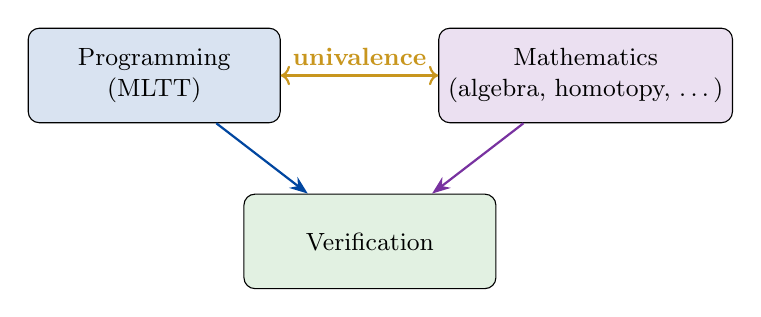
\begin{tikzpicture}[
    box/.style={draw,rounded corners,minimum width=3.2cm,
                minimum height=1.2cm,align=center,font=\small},
    arr/.style={-Stealth,thick}
  ]
    \node[box,fill=emphblue!15] (prog) {Programming\\(MLTT)};
    \node[box,fill=hottviolet!15,right=2.0cm of prog] (math)
      {Mathematics\\(algebra, homotopy, \ldots)};
    \node[box,fill=cubgreen!15,below=1.5cm of $(prog)!0.5!(math)$] (verif)
      {Verification};
    \draw[arr,emphblue] (prog) -- (verif);
    \draw[arr,hottviolet] (math) -- (verif);
    \draw[arr,equivgold,<->] (prog) -- (math)
      node[midway,above,font=\small\bfseries,text=equivgold]{univalence};
  \end{tikzpicture}
  \end{center}
  \pause\medskip
  \textbf{Lingua franca}: program as in MLTT, import higher concepts from mathematics,
  verify with both in the same language.
\end{frame}

% ---- Cubical vs Coq positioning ----------------------------
%\begin{frame}{Positioning: Cubical Agda vs.\ Coq / Lean}
%  \begin{center}
%  \begin{tabular}{lcc}
%    \toprule
%    Feature & \textbf{Coq / Lean} & \textbf{Cubical Agda} \\
%    \midrule
%    Equality & intensional & \alert{cubical (CCHM)} \\
%    Univalence & axiom / inconsistent & \alert{computes} \\
%    HITs & encoded / partial & \alert{native} \\
%    Quotient types & setoid hell & \alert{built-in} \\
%    Tactics & rich ecosystem & limited \\
%    Library size & large & growing \\
%    \bottomrule
%  \end{tabular}
%  \end{center}
%  \pause\medskip
%  Not a replacement but a \emph{complement}. \\
%  Different sweet spot: mathematics-heavy formalization.
%\end{frame}

% ############################################################
% PART 2: CORE IDEAS  (~15 min, ~7 slides)
% ############################################################

\sectionframe{Part 2\\[4pt] \large Univalence and the Structure Identity Principle}

% ---- Path types --------------------------------------------
\begin{frame}{Identity types, cubically}
  In cubical type theory, an identity (``path'') $p : a = b$
  is a function from the \emph{interval} $\mathbb{I}$:
  \[
    p : \mathbb{I} \to A
    \qquad p(\mathtt{i0}) \;=\; a
    \qquad p(\mathtt{i1}) \;=\; b
  \]
  \pause\medskip
  \begin{center}
  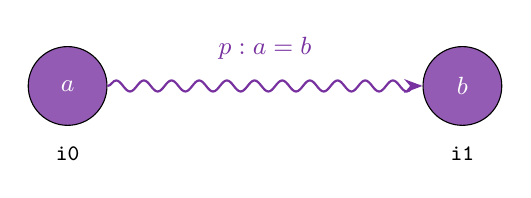
\begin{tikzpicture}
    \node[ndA,minimum size=10mm] (a) {$a$};
    \node[ndA,minimum size=10mm,right=4cm of a] (b) {$b$};
    \draw[-Stealth,thick,hottviolet,decorate,
          decoration={snake,amplitude=2pt,segment length=10pt}]
      (a) -- (b) node[midway,above=6pt,font=\small]{$p : a = b$};
    \node[below=4pt of a,lbl]{$\mathtt{i0}$};
    \node[below=4pt of b,lbl]{$\mathtt{i1}$};
  \end{tikzpicture}
  \end{center}
  \pause\medskip
  Key consequence: $\transp$ along paths \emph{computes}.
\end{frame}

% ---- Univalence -------------------------------------------
\begin{frame}{Univalence}
  \begin{block}{Univalence axiom (Voevodsky, 2006)}
    The canonical map
    $(A = B) \to (A \simeq B)$
    is itself an equivalence:
    \[
      (A =_\U B) \;\simeq\; (A \simeq B)
    \]
  \end{block}
  \pause\medskip
  In Cubical Agda this is not an axiom but a \emph{theorem}:

  \medskip
  \texttt{ua \ \ : A $\simeq$ B $\to$ A $=$ B}\\
  \texttt{ua-$\beta$ : transport (ua e) x $=$ e .fst x}\\
  \texttt{ua-$\eta$ : ua ($=\to\simeq$ p) $=$ p}
  \pause\medskip

  \textbf{Caveat:}
  In the current implementation of Cubical Agda anything transported
  through $ua$ has to be marked as \underline{erased}.
\end{frame}

% ---- Transport in action ----------------------------------
\begin{frame}{Transport in action: predicate transfer}
  Suppose we have:
  \begin{itemize}
    \item $e : \mathbb{N} \simeq \mathrm{Bin}$
      \quad (from \texttt{$\mathbb{N}\to$Bin} / \texttt{Bin$\to\mathbb{N}$})
    \item $\mathit{IsEven} : \mathbb{N} \to \mathcal{U}$
  \end{itemize}
  \pause\medskip
  Then:

  \medskip
  \texttt{IsEvenB : Bin $\to$ $\mathcal{U}$}\\
  \texttt{IsEvenB = transport ($\lambda$ i $\to$ ua e i $\to$ $\mathcal{U}$) IsEven}

  \pause\medskip
  And any theorem \texttt{thm : ($\forall$ n $\to$ IsEven n $\to$ P n)} transports the same way:

  \medskip
  \texttt{thm' : $\forall$ b $\to$ IsEvenB b $\to$ P' b}\\
  \texttt{thm' = transport ($\ldots$\ ua e $\ldots$) thm}

\end{frame}

% ---- SIP motivation ----------------------------------------
\begin{frame}{From bare to structured types: the SIP}
  Univalence says that equivalent \emph{types} are equal. \\
  But we usually work with \emph{structures} (monoids, rings, queues, \ldots).
  \pause\bigskip

  \begin{block}{Structure Identity Principle (SIP)}
    Two structured types $(A, s_A)$ and $(B, s_B)$ are equal \\
    iff there is an equivalence $e : A \simeq B$ that \emph{preserves the structure}:
    \[
      (A, s_A) = (B, s_B)
      \;\;\simeq\;\;
      \Sigma(e : A \simeq B).\; s_A =_{e} s_B
    \]
  \end{block}
  \pause\medskip
  This is representation independence built into the type theory.
\end{frame}

% ---- SIP example -------------------------------------------
\begin{frame}{SIP in practice: monoids on $\mathbb{N}$ and \texttt{Bin}}
  A \textbf{monoid structure} on a carrier $T$ is
  \[
    \mathrm{MonStr}(T) \;=\; \Sigma(e : T).\; \Sigma(\_\!\cdot\!\_\, : T \to T \to T).\;
    \mathrm{Axioms}(e, \cdot)
  \]
  \pause\medskip

  \textbf{Impl 1:} $(\mathbb{N},\, 0,\, +)$ \qquad
  \textbf{Impl 2:} $(\mathrm{Bin},\, \mathtt{BinO},\, \mathtt{binPlus})$

  \medskip
  The equivalence $\mathbb{N} \simeq \mathrm{Bin}$ is a
  \emph{monoid homomorphism} (\texttt{$\mathbb{N}\to$Bin-+}),
  so by SIP:
  \[
    p : (\mathbb{N},0,+) \;=\; (\mathrm{Bin},\mathtt{BinO},\mathtt{binPlus})
    \quad \text{as structured types.}
  \]

  \pause\medskip
  \textbf{Conicity} (no nontrivial zero sums) is a property of the monoid:
  \[
    \mathrm{Conical}(T,e,\cdot) \;=\;
    \forall (x\,y : T) \to\; x \cdot y = e \;\to\; (x = e) \times (y = e)
  \]

  \pause\medskip
  Prove once for $(\mathbb{N},0,+)$, then transport:

  \smallskip
  \texttt{conical-Bin : Conical Bin-monoid}\\
  \texttt{conical-Bin = transport ($\lambda$ i $\to$ Conical (p i)) conical-$\mathbb{N}$}
\end{frame}

% ---- SIP for Coq engineers --------------------------------
% \begin{frame}{What SIP replaces in Coq}
%   \begin{columns}[T]
%     \begin{column}{0.48\textwidth}
%       \textbf{In Coq / VST:}
%       \begin{itemize}
%         \item Define abstract spec
%         \item Define concrete impl
%         \item Prove refinement relation
%         \item Manually apply \texttt{transfer} \\
%               at every use site
%         \item Repeat for each new impl
%       \end{itemize}
%     \end{column}
%     \pause
%     \begin{column}{0.48\textwidth}
%       \textbf{In Cubical Agda:}
%       \begin{itemize}
%         \item Define the structure
%         \item Prove the equivalence \emph{once}
%         \item SIP gives you: \\
%               \alert{all theorems transfer} \\
%               \alert{all programs swap} \\
%               automatically
%       \end{itemize}
%     \end{column}
%   \end{columns}
% \end{frame}

% ############################################################
% PART 3: Truncation and Quotients  (~10 min, ~4 slides)
% ############################################################

\sectionframe{Part 3\\[4pt] \large Truncation and Quotients}

% ---- Truncation levels overview ----------------------------
\begin{frame}{The h-level hierarchy}
  Types in HoTT have a \emph{truncation level} (``h-level''):
  \medskip
  \begin{center}
  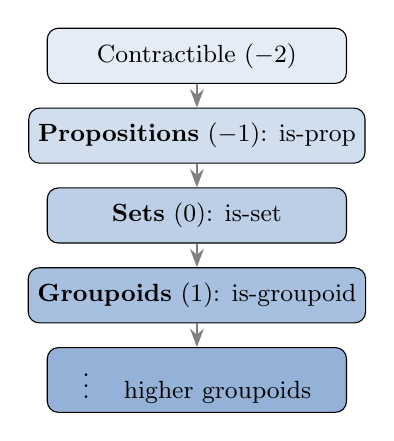
\begin{tikzpicture}[
    lvl/.style={draw,rounded corners,minimum width=3.8cm,
                minimum height=0.7cm,align=center,font=\small},
    arr/.style={-Stealth,thick,black!50}
  ]
    \node[lvl,fill=emphblue!10] (contr) at (0,0)
      {Contractible ($-2$)};
    \node[lvl,fill=emphblue!18,below=0.3cm of contr] (prop)
      {\textbf{Propositions} ($-1$): $\isProp$};
    \node[lvl,fill=emphblue!26,below=0.3cm of prop] (set)
      {\textbf{Sets} ($0$): $\isSet$};
    \node[lvl,fill=emphblue!34,below=0.3cm of set] (gpd)
      {\textbf{Groupoids} ($1$): $\isGroupoid$};
    \node[lvl,fill=emphblue!42,below=0.3cm of gpd] (dots)
      {$\vdots$ \quad higher groupoids};
    \draw[arr] (contr) -- (prop);
    \draw[arr] (prop) -- (set);
    \draw[arr] (set) -- (gpd);
    \draw[arr] (gpd) -- (dots);
  \end{tikzpicture}
  \end{center}
  \pause\medskip
  Most ``ordinary'' mathematics lives at levels $-1$ (props) and $0$ (sets). \\
  Groupoids appear in higher-dimensional algebra, logic and concurrency.
\end{frame}

% ---- Propositional truncation ------------------------------
\begin{frame}{Propositional truncation: ``mere existence''}
  \begin{block}{Propositional truncation}
    $\trunc{A}$ is $A$ with all paths between inhabitants identified:
    \[
      \trunc{A} : \mathcal{U}
      \qquad
      \tmark{\cdot} : A \to \trunc{A}
      \qquad
      trunc : \isProp(\trunc{A})
    \]
  \end{block}
  \pause\medskip
  \textbf{Meaning:} ``$A$ is inhabited'' without choosing a witness.
  \pause\medskip

  \textbf{Why it matters:}
  \begin{itemize}
    \item Mathematicians say ``there exists'' without constructing a witness
    \item In raw MLTT, $\Sigma$-types give \emph{specific} witnesses
    \item $\trunc{\Sigma\ldots}$ recovers classical-style
          existential statements
  \end{itemize}
\end{frame}

% ---- Truncation in action: surjectivity (1/2) --------------
\begin{frame}{Truncation in action: split vs.\ classical surjectivity}
  Two notions of ``$f : A \to B$ is surjective'':
  \pause\medskip

  \begin{block}{Split-surjective ($A \twoheadrightarrow ! \ B$) --- a \emph{structure}}
    \[
      \mathrm{SplitSurj}(f) \;=\; \forall(y : B).\; \mathrm{fibre}\;f\;y
      \;=\; \forall(y : B).\; \Sigma(x : A).\; f\;x = y
    \]
    A \emph{function} that produces a preimage --- exhibits $f$ as a retraction
    (left inverse).
  \end{block}
  \pause

  \begin{block}{Surjective ($A \twoheadrightarrow B$) --- a \emph{property}}
    \[
      \mathrm{Surj}(f) \;=\; \forall(y : B).\; \trunc{\mathrm{fibre}\;f\;y}
    \]
    Each fibre is merely inhabited; $\mathrm{Surj}(f)$ is a proposition.
  \end{block}
\end{frame}

% ---- Truncation in action: surjectivity (2/2) --------------
\begin{frame}{Structure vs.\ property: why $\trunc{-}$ matters}
  \textbf{In raw MLTT these notions collapse:} \\
  $\Sigma$ always carries a specific witness, so ``there exists''
  means ``here is one.''
  \pause\medskip

  \textbf{With $\trunc{-}$:} one recovers the \emph{classical} reading
  (``$f$ hits every point'') without committing to a chosen right inverse.
  \pause\medskip

  In fact, the classical existential quantifier is definable as
  \[
    \exists (A : \mathcal{U})\;(B : A \to \mathcal{U}) \;:=\; \trunc{\Sigma\,A\,B}
  \]
  \pause\medskip

  So:\\
  \textbf{split-surjective} $=$ ``$\forall y.\ \Sigma x.\ f\,x = y$'' (data); \\
  \textbf{surjective} $=$ ``$\forall y.\ \exists x.\ f\,x = y$'' (proposition).
\end{frame}

% ---- LFSet: listed finite sets as a HIT --------------------
\begin{frame}{Listed finite sets as a HIT}
  Finite subsets of \texttt{A}, built as cons-lists
  \emph{quotiented} by ``no duplicates, no order'':
  \medskip

  \begin{center}
  \begin{tabular}{l}
  \texttt{data LFSet (A : $\mathcal{U}$) : $\mathcal{U}$ where}\\
  \texttt{\ \ []\ \ \ : LFSet A}\\
  \texttt{\ \ \_::\_\ : A $\to$ LFSet A $\to$ LFSet A}\\
  \texttt{\ \ drop\ : x :: x :: xs\ \ \ $=$\ \ x :: xs}\\
  \texttt{\ \ swap\ : x :: y :: xs\ \ \ $=$\ \ y :: x :: xs}\\
  \texttt{\ \ trunc : is-set (LFSet A)}
  \end{tabular}
  \end{center}
  \pause\medskip

  This is a \emph{higher inductive type} (HIT): path constructors \texttt{drop}/\texttt{swap} identify lists that
  represent the same set. \texttt{trunc} truncates to a set
  (no higher coherences).

  \pause\medskip
  \textbf{No setoid discipline:} functions out of \texttt{LFSet A} must
  respect \texttt{drop} and \texttt{swap} --- enforced on elimination by the type checker directly,
  not by external mechanisms.
\end{frame}

% ---- LFSet membership --------------------------------------
\begin{frame}{Membership: combining ua and $\trunc{-}$}
  Define \texttt{\_$\in$\_ : A $\to$ LFSet A $\to$ Prop} by recursion:
  \medskip

  \begin{center}
  \begin{tabular}{l}
  \texttt{x $\in$ []\ \ \ \ \ \ \ \ \ = $\bot$}\\
  \texttt{x $\in$ (y :: xs) = (x $=$ y) $\lor$ (x $\in$ xs)}
  \end{tabular}
  \end{center}
  \pause\medskip

  For \texttt{\_$\in$\_} to be a \emph{relation on the HIT}, it must respect
  \texttt{drop} and \texttt{swap}:
  \medskip

  \begin{itemize}
    \item \texttt{drop}: \ $(x = y) \lor (x = y) \lor P \;=\; (x = y) \lor P$
    \item \texttt{swap}: \ $(x = y) \lor (x = z) \lor P \;=\; (x = z) \lor (x = y) \lor P$
  \end{itemize}
  \pause\medskip

  These are type equalities, obtained by:
  \begin{itemize}
    \item $\trunc{-}$ --- to define $\lor$ as $\trunc{\_ \uplus \_}$,
          making it idempotent and commutative \emph{up to equivalence};
    \item \emph{univalence} --- to turn those equivalences into
          the paths demanded by \texttt{drop}/\texttt{swap}.
  \end{itemize}
\end{frame}

% ############################################################
% PART 4: THE ZOO OF FINITE SETS  (~10 min, ~5 slides)
% ############################################################

\sectionframe{Part 4\\[4pt] \large The Zoo of Finite Sets}

% ---- Many notions of finiteness ----------------------------
\begin{frame}{How many ways can a set be finite?}
  \begin{center}
  \begin{tabular}{ll}
    \toprule
    \textbf{Name} & \textbf{Definition} \\
    \midrule
    Split-enumerable &
      $\Sigma(n:\mathbb{N})\; \Fin\;n \twoheadrightarrow ! A$ \\[3pt]
    Bishop-finite &
      $\Sigma(n:\mathbb{N})\; \Fin\;n \simeq A$ \\[3pt]
    Cardinal-finite &
      $\exists(n:\mathbb{N})\; \Fin\;n \simeq A$ \\[3pt]
    Manifest-enumerable &
      $\Sigma(n:\mathbb{N})\; \Fin\;n \twoheadrightarrow A$ \\[3pt]
    Kuratowski-finite &
      $\exists(n:\mathbb{N})\; \Fin\;n \twoheadrightarrow A$ \\[3pt]
    Dedekind-finite &
      $\forall(f:X \to X) \to \mathrm{is\text{-}embedding}\ f \to \isEquiv\ f$ \\[3pt]
    \ldots & \ldots \\
    \bottomrule
  \end{tabular}
  \end{center}
  \pause\medskip
  In classical math these (mostly) coincide. \\
  Constructively they form a \emph{hierarchy} of distinct notions.
\end{frame}

% ---- Structure vs property in finiteness -------------------
\begin{frame}{Which finiteness should I use?}
  These notions differ by how much \emph{structure} on the carrier
  they demand:
  \begin{itemize}
    \item \textbf{Bishop-finite} / \textbf{Split-enumerable}: a chosen
          enumeration $\Rightarrow$ \emph{decidable equality} and an
          induced \emph{ordering}.
    \item \textbf{Manifest-enumerable}: a chosen surjection from
          $\Fin\;n$ (possibly with duplicates) $\Rightarrow$ induces a
          \emph{total order}, but \emph{no} decidable equality.
    \item \textbf{Cardinal-finite}: an enumeration \emph{merely exists}
          $\Rightarrow$ decidable equality, but no canonical order.
    \item \textbf{Kuratowski-finite}: a surjection from $\Fin\;n$
          merely exists $\Rightarrow$ \emph{no} decidable equality nor ordering.
  \end{itemize}
  \pause\medskip

  \textbf{In practice:} \textbf{Kuratowski} and \textbf{cardinal} are the
  two most useful.
  \begin{itemize}
    \item \textbf{Kuratowski} is the weakest (basic building block).
    \item \textbf{Cardinal} $=$ \textbf{Kuratowski} $+$ decidable equality.
  \end{itemize}
  \pause\medskip

  In HoTT the universe of finite types is \emph{itself} a rich object.
\end{frame}

% ---- FinSet n -------------------------------------------
\begin{frame}{The universe of $n$-element sets}
  \[
    \mathrm{FinSet}_n \;\triangleq\;
    \Sigma(X : \U)\; \trunc{X \simeq \Fin\;n}\;
    \simeq \exists(X : \U)\; X \simeq \Fin\;n\;
  \]
  \pause\medskip
  \textbf{What is this type?}
  \begin{itemize}
    \item Objects: types that are merely equivalent to $\Fin\;n$
    \item Paths: \emph{equivalences} between them (by univalence!)
    \item $\Rightarrow$ loop space $\Omega(\mathrm{FinSet}_n) \simeq \mathrm{Aut}(\Fin\;n) \simeq S_n$
  \end{itemize}
  \pause\medskip
  \begin{center}
    $\mathrm{FinSet}_n$ is the \emph{classifying space} $B S_n$ \\
    of the symmetric group $S_n$!
  \end{center}
  \pause\medskip
  Finite sets themselves form a \emph{groupoid}.
\end{frame}

% ---- Why this matters --------------------------------------
\begin{frame}{Why does groupoid structure matter?}
  In set-level type theory:
  \begin{itemize}
    \item $\Fin\;3 = \Fin\;3$ has \emph{one} proof: $\refl$
    \item Symmetries are invisible
  \end{itemize}
  \pause\medskip
  In HoTT:
  \begin{itemize}
    \item $\Fin\;3 = \Fin\;3$ has \emph{six} proofs: $|S_3|$
    \item Can reason about orbits, stabilizers, Burnside's lemma, \ldots
  \end{itemize}
  \pause\medskip
  \textbf{Applications:} combinatorics;
  verifiable shuffles in cryptography;
  unordered containers (bags, multisets);
  Joyal species / polynomial functors.
\end{frame}

% ---- Small universes of FinSets ----------------------------
\begin{frame}{Small universes and FinSet}
  Finite types assemble into a \emph{small universe}:
  \[
    \mathrm{FinSet} \;\triangleq\;
    \Sigma(n : \mathbb{N})\; \mathrm{FinSet_n}
  \]
  \pause\medskip
  This universe has:
  \begin{itemize}
    \item Coproducts, products, function types (when finite)
    \item A natural ``cardinality'' map $\mathrm{FinSet} \to \mathbb{N}$
    \item Rich path structure: $\mathrm{FinSet} \simeq \coprod_n B S_n$
  \end{itemize}
  \pause\medskip

  \pause\medskip
  Useful building block for finite-dimensional linear algebra, \\
  finite probability, reversible computation, \ldots
\end{frame}

% ---- Diagram: FinSet structure  ----------------------------
\begin{frame}{Structure of $\mathrm{FinSet}$}
  \begin{center}
  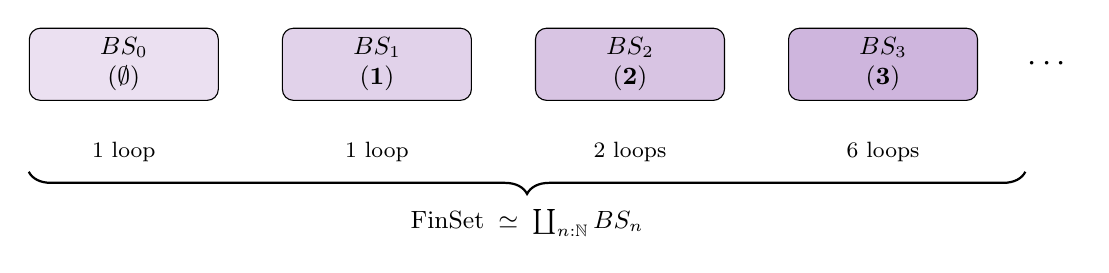
\begin{tikzpicture}[
    comp/.style={draw,rounded corners,minimum width=2.4cm,
                 minimum height=0.9cm,align=center,font=\small},
  ]
    \node[comp,fill=hottviolet!15] (bs0) {$B S_0$\\($\emptyset$)};
    \node[comp,fill=hottviolet!22,right=0.8cm of bs0]
      (bs1) {$B S_1$\\($\mathbf{1}$)};
    \node[comp,fill=hottviolet!29,right=0.8cm of bs1]
      (bs2) {$B S_2$\\($\mathbf{2}$)};
    \node[comp,fill=hottviolet!36,right=0.8cm of bs2]
      (bs3) {$B S_3$\\($\mathbf{3}$)};
    \node[right=0.5cm of bs3,font=\large] {$\cdots$};
    % loop annotations
    \node[below=0.4cm of bs0,lbl]{1 loop};
    \node[below=0.4cm of bs1,lbl]{1 loop};
    \node[below=0.4cm of bs2,lbl]{2 loops};
    \node[below=0.4cm of bs3,lbl]{6 loops};
    % big brace
    \draw[decorate,decoration={brace,amplitude=8pt,mirror},thick]
      ($(bs0.south west)+(0,-0.9)$) -- ($(bs3.south east)+(0.6,-0.9)$)
      node[midway,below=10pt,font=\small]
      {$\mathrm{FinSet} \;\simeq\; \coprod_{n:\mathbb{N}} B S_n$};
  \end{tikzpicture}
  \end{center}
\end{frame}

% ############################################################
% PART 5: CODE TOUR --- SYMMETRY BOOK  (~10 min, ~5 slides)
% ############################################################

\sectionframe{Part 5\\[4pt] \large The \emph{Symmetry} Book}

% ---- Symmetry book overview --------------------------------
\begin{frame}{The \emph{Symmetry} book}
  {\small Bezem, Buchholtz, Cagne, Dundas, Grayson}
  \medskip

  A textbook on group theory \emph{from the HoTT perspective}, \\
  formalization in Cubical Agda WIP.
  \pause\medskip

  \textbf{Key idea:} a group is not an algebraic structure. \\
  A group \emph{is} a pointed connected groupoid:
  \[
    \BG \;\triangleq\;
    \Sigma(X : \U).\; \trunc{X} \times (\forall\ (x\ y : X) \to \trunc{x = y}) \times \isGroupoid(X)
  \]
  \pause\medskip
  \begin{itemize}
    \item Elements of $G$: loops at the base point
    \item Group operation: path composition
    \item Inverse: path reversal
    \item Axioms: \emph{automatic}, from path algebra
  \end{itemize}
\end{frame}

% ---- Groups as groupoids: picture -------------------------
\begin{frame}{Groups as groupoids: the delooping picture}
  \begin{center}
  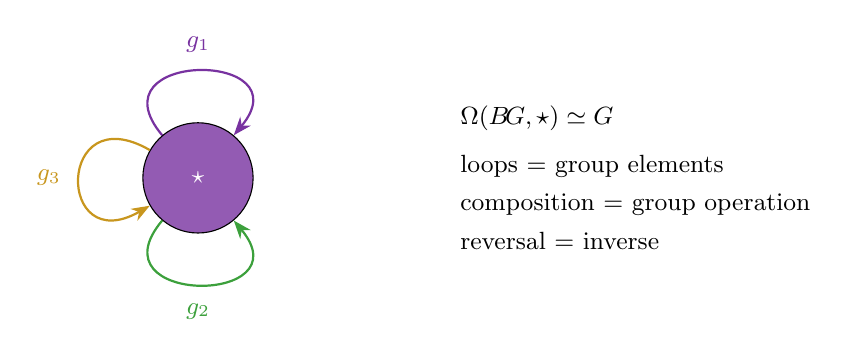
\begin{tikzpicture}
    % The pointed connected groupoid
    \node[ndA,minimum size=14mm] (pt) {$\star$};
    % loops
    \draw[-Stealth,thick,hottviolet,out=130,in=50,looseness=4]
      (pt) to node[above=3pt,font=\small]{$g_1$} (pt);
    \draw[-Stealth,thick,cubgreen,out=230,in=310,looseness=4]
      (pt) to node[below=3pt,font=\small]{$g_2$} (pt);
    \draw[-Stealth,thick,equivgold,out=150,in=210,looseness=5]
      (pt) to node[left=3pt,font=\small]{$g_3$} (pt);
    % label
    \node[right=2.5cm of pt,align=left,font=\small] {
      $\Omega(\BG, \star) \simeq G$ \\[6pt]
      loops $=$ group elements \\[3pt]
      composition $=$ group operation \\[3pt]
      reversal $=$ inverse
    };
  \end{tikzpicture}
  \end{center}
  \pause\medskip
  A \textbf{group homomorphism} $G \to H$ is just a \emph{pointed map} $\BG \to B\!H$.

  \pause\medskip
  A \textbf{group action} of $G$ on a set $X$
  is a map $\BG \to Set$.

  \pause\medskip
  No coherence conditions to check --- the type theory handles them.
\end{frame}

% ---- Code example: defining a group -----------------------
\begin{frame}{Code: defining a group in Cubical Agda}
  \texttt{-{}- A group is a pointed connected groupoid}\\
  \texttt{Group : }$\mathcal{U}_1$\\
  \texttt{Group = }$\Sigma$\texttt{(BG : }$\mathcal{U}$\texttt{)}\\
  \texttt{\ \ \ \ \ \ \ \ }$\times$\texttt{\ is-connected BG}\\
  \texttt{\ \ \ \ \ \ \ \ }$\times$\texttt{\ is-groupoid BG}\\[6pt]
  \texttt{-{}- The underlying shape of a group (as a set)}\\
  \texttt{sh : Group }$\to$\texttt{ }$\mathcal{U}$\\
  \texttt{sh BG = (pt BG == pt BG)}
  \pause\medskip

  Compare with the classical definition: carrier, operation, unit,
  inverse, three axioms, \ldots
\end{frame}

% ---- Code example: group actions ---------------------------
\begin{frame}{Code: group actions}
  \texttt{-{}- An action of G on sets is a map BG }$\to$\texttt{ Set}\\
  \texttt{Action : Group }$\to$\texttt{ }$\mathcal{U}_1$\\
  \texttt{Action G = BG G }$\to$\texttt{ Set}\\[6pt]
  \texttt{-{}- The orbit type}\\
  \texttt{Orbit : \{G : Group\} }$\to$\texttt{ Action G }$\to$\texttt{ }$\mathcal{U}$\\
  \texttt{Orbit \{G\} X = }$\Sigma$\texttt{(b : BG G) }$\times$\texttt{ X b}
  \pause\medskip

  Orbit-stabilizer, Burnside, \ldots\ all follow from
  the path algebra of $\BG$.

  \pause\medskip
  Main win is compactness: pages of algebraic boilerplate become a few lines.
\end{frame}

% ---- What computes? ----------------------------------------
\begin{frame}{Does it actually compute?}
  Yes --- but with proof-engineering work:
  \begin{itemize}
    \item $\transp$ along $\ua$ reduces, but you often have to invoke
          \texttt{ua-}$\beta$ \emph{by hand} at the right place to keep
          goals tractable
    \item HITs reduce via Kan operations, but for anything beyond toy
          examples you write \emph{custom eliminators} so proofs read
          like ordinary recursion
    \item Composition of cubes is combinatorially expensive ---
          performance is a real concern at scale
  \end{itemize}
  \pause\medskip
  Despite all that: chapters 2-3 (and parts of 4) of \emph{Symmetry} book type-check
  (thousands of lines), there are many examples of libraries: \texttt{cubical}, \texttt{1lab}, \texttt{cubical-mini}.
\end{frame}

% ---- Plug: cubical-mini -----------------------------------
\begin{frame}{Shameless plug: \href{https://github.com/cmcmA20/cubical-mini}{\texttt{cubical-mini}}}
  A custom Cubical Agda library we've been developing for the past
  $\sim$3 years.
  \pause\medskip

  \textbf{Lineage:} a mix of ideas from
  \begin{itemize}
    \item the standard \href{https://github.com/agda/cubical/}{\texttt{cubical}} library,
    \item the \href{https://1lab.dev/}{\texttt{1lab}},
    \item Escard\'o's \href{https://martinescardo.github.io/TypeTopology/}{\texttt{TypeTopology}},
    \item and a dose of Coq's \href{https://math-comp.github.io/}{\texttt{mathcomp} / \texttt{ssreflect}} style.
  \end{itemize}
  \pause\medskip

  \textbf{Design choices:}
  \begin{itemize}
    \item \texttt{-{}-erased-cubical} on by default
    \item No axioms (in particular, no propositional resizing)
    \item Tries to balance \emph{mathematical readability} with
          \emph{practical proof engineering}
  \end{itemize}
  \pause\medskip

  \textbf{v2 in the works:}
  \href{https://github.com/cubical-mini/core/}{\texttt{cubical-mini/core}}
  --- instead of using Agda primitives directly, expose them as
  \emph{instances} of a few abstract interfaces. The core acts as an
  insulation layer, shielding downstream code from the arbitrariness
  of the usual stdlib interfaces.
\end{frame}

% ############################################################
% PART 6: WRAP-UP & DISCUSSION  (~5 min, ~2 slides)
% ############################################################

\sectionframe{Part 6\\[6pt]Wrap-Up \& Discussion}

% ---- Summary ----------------------------------------------
\begin{frame}{Summary}
  \begin{enumerate}
    \item[\textbf{1.}] \textbf{Univalence eliminates boilerplate}
    \begin{itemize}
      \item Equivalent types are equal, transport is free
    \end{itemize}
    \pause\medskip
    \item[\textbf{2.}] \textbf{SIP gives representation independence for free}
    \begin{itemize}
      \item Prove equivalence once, reuse everything
    \end{itemize}
    \pause\medskip
    \item[\textbf{3.}] \textbf{Truncation \& quotients keep math comfortable}
    \begin{itemize}
      \item Mere existence, quotient \& higher inductive types --- no setoid hell
    \end{itemize}
    \pause\medskip
    \item[\textbf{4.}] \textbf{The universe is richer than in MLTT}
    \begin{itemize}
      \item Groupoid structure lets you reason about symmetries
      \item FinSets, classifying spaces, higher group theory
    \end{itemize}
    \pause\medskip
    \item[\textbf{5.}] \textbf{It all computes}
    \begin{itemize}
      \item No axioms, the cubical evaluator handles it
    \end{itemize}
  \end{enumerate}
\end{frame}

% ---- Future directions ------------------------------------
\begin{frame}{Future directions}
  \begin{enumerate}
    \item[\textbf{1.}] \textbf{Modal type theories.}
      Modalities interact nicely with the interval. Two families
      currently implemented:
      \begin{itemize}
        \item \emph{Guarded types} --- reasoning about productivity,
              corecursive / potentially infinite / lazy algorithms
              with type-directed coinduction.
        \item \emph{Spatial types} --- synthetic topology.
      \end{itemize}
    \pause\medskip
    \item[\textbf{2.}] \textbf{Discrete differential geometry} \`a la Langmead
      \\ {\small
      \href{https://greg.langmead.info/writing/differential_geometry_in_hott/}%
           {"Discrete differential geometry in homotopy type theory"}}
      constructs connections, curvature, and vector fields, proves 2-dimensional version of discrete Gauss-Bonnet-Poincaré theorem.
  \end{enumerate}
\end{frame}

% ---- Open questions ----------------------------------------
\begin{frame}{Open questions}
  \begin{itemize}
    \item Can SIP / univalence simplify \textbf{VST-style verification}? \\
          {\small (representation changes in low-level program proofs)}
    \pause\medskip
    \item Can \textbf{proof search} exploit the richer structure of cubical types?
    \pause\medskip
    \item \textbf{Interoperability:} can we transfer results between Coq/Lean formalizations and Cubical Agda? \\
    {\small (impredicativity / classicality pose challenges)}
    \pause\medskip
    \item \textbf{Performance:} when will cubical evaluation \\
          be practical for large-scale verification?
          (upcoming Agda 2.9.0 has some impressive optimizations already)
  \end{itemize}
  \pause\bigskip
  \begin{center}
    {\Huge\bfseries Thank you!}
  \end{center}
\end{frame}

% ============================================================
\appendix
\section*{Extra slides}
% ============================================================

% ---- CCHM operations --------------------------------------
\begin{frame}{Appendix: CCHM in a nutshell}
  Cubical type theory (Cohen, Coquand, Huber, M\"{o}rtberg, 2018):
  \medskip
  \begin{itemize}
    \item \textbf{Interval} $\mathbb{I}$ with endpoints $\mathtt{i0}, \mathtt{i1}$
    \item \textbf{Path types:} $\mathrm{PathP}\;(\lambda\,i.\;A\;i)\;a\;b$
    \item \textbf{Kan operations:} $\mathrm{hcomp}$ (composition)
          and $\mathrm{transp}$ (transport)
    \item \textbf{Glue types:} the mechanism behind $\ua$
  \end{itemize}
  \medskip
  All operations are \emph{computational} (reduce during type-checking).
\end{frame}

% ---- References -------------------------------------------
\begin{frame}{References}
  \small
  \begin{itemize}
    \item Rijke, \emph{Introduction to Homotopy Type Theory}, 2022.
          \href{https://arxiv.org/abs/2212.11082}{arXiv:2212.11082}
    \item HoTT Book, \emph{Homotopy Type Theory}, 2013
    \item Cohen, Coquand, Huber, M\"{o}rtberg,
          \emph{Cubical Type Theory}, 2018
    \item Vezzosi, M\"{o}rtberg, Abel,
          \emph{Cubical Agda}, ICFP 2019
    \item Angiuli, Cavallo, M\"{o}rtberg, Zeuner,
          \emph{Internalizing Representation Independence \\
          with Univalence}, POPL 2021
    \item Bezem, Buchholtz, Cagne, Dundas, Grayson,
          \emph{Symmetry}, 2025+
    \item \texttt{cubical-mini} library:
          \url{https://github.com/cmcmA20/cubical-mini/}
  \end{itemize}
\end{frame}

\end{document}
